\documentclass[a4paper,12pt]{report}

\usepackage[dutch]{babel}           % Nederlands
\usepackage[latin1]{inputenc}       % speciale karakters

\usepackage{palatino} % font
\usepackage{graphicx} % figuren
\usepackage{float}
%\graphicspath{{}}
\usepackage{subcaption}

\usepackage[hyperfootnotes=false]{hyperref} % PDF bookmarks
\usepackage{titlesec}	
\usepackage{fancyhdr}

\renewenvironment{quote}                            % kleinere citaten
               {\list{}{\rightmargin\leftmargin}    %
                \item[]\small}                      %
               {\endlist}                           %

\setlength{\parindent}{0pt}         % indenteringen met witlijn
\setlength{\parskip}{1em}           %

\setlength{\hoffset}{-1cm}          % kleinere marges
\addtolength{\textwidth}{2cm}
\setlength{\voffset}{-1cm}
\addtolength{\textheight}{2cm}

\makeatletter                               % een witlijn tussen
\renewcommand{\footnoterule}{               % voetnoten en tekst
  \vspace{1em}                              %
  \kern-3\p@\hrule\@width.4\columnwidth     %
  \kern2.6\p@}                              %
\makeatother                                %
                                            %
                               
\usepackage[stable]{footmisc}               % pakket voor bep. voetnoten. (voetnoten in titels)

\usepackage{graphicx}   %afbeeldingen

\newcommand{\nroman}{\renewcommand{\thepage}{\roman{page}}\setcounter{page}{0}}     % romeinse nummers
\newcommand{\narabic}{\renewcommand{\thepage}{\arabic{page}}\setcounter{page}{1}}   % arabische nummers


%\bibliographystyle{plain}
%\usepackage[nottoc,section]{tocbibind}     % bibliografie in TOC, sectiegrootte
\setcounter{tocdepth}{3}                   % diepte van de TOC

\usepackage[linesnumbered,ruled,vlined]{algorithm2e} 		% Algoritmen
\usepackage{algpseudocode}
\renewcommand*{\listalgorithmcfname}{Lijst van algoritmen}	%
\renewcommand*{\algorithmcfname}{Algoritme}					%
\renewcommand*{\algorithmautorefname}{algoritme}	

\SetKwInput{KwData}{Data}
\SetKwInput{KwResult}{Resultaat}

\lhead{Brent Van Wynsberge}
\rhead{Project Algoritmen en Datastructuren III}




%%% TITEL EN AUTEUR %%%

\renewcommand{\title}{%
			Huffman compressie \\
			\large Project Algoritmen en Datastructuren III}
\renewcommand{\author}{
\textbf{\large Brent Van Wynsberge} \\
\small 3$^e$ bachelor Informatica, Universiteit Gent \\
\small Algoritmen en Datastructuren III \\
\small Stamnummer: 01201853 \\
}

%%% / / / %%%

\renewcommand{\maketitle}{
\thispagestyle{empty}
\begin{minipage}{3.5in}

\includegraphics{ugent.png}
\end{minipage}
\hfill
\begin{minipage}{3in}
\begin{flushright}
\author
\bigskip
\textbf{\today}
\end{flushright}
\end{minipage}
\vspace{5em}
\vspace*{\fill}
\begin{center}
\Huge{\title}
\end{center}
\vspace*{\fill}}

\titleformat{\chapter}{\normalfont\huge}{\thechapter.}{20pt}{\huge} %chapterformat
\newcommand{\bigO}[1]{$\bm{\mathcal{O}(#1)}$} %big O notatie
\newcommand{\pp}[0]{\texttt{++}}
\usepackage{bm}
\newcommand\ceil[1]{\lceil#1\rceil}

\usepackage{fixltx2e} %images??
\MakeRobust{\Call}

\begin{document}
\global\emergencystretch = .3\hsize

%%% INLEIDEND %%%
\nroman
\maketitle
\newpage

\tableofcontents
\newpage

\pagestyle{fancy}

%%% HOOFDSTUKKEN %%%
%%%%%%%%%%%%%\input{algemeen}
\newpage
\narabic

\chapter{Algoritmen}
In dit onderdeel bekijken we de pseudocode van alle ge\"implementeerde algoritmen. Wanneer er een niet triviale operatie opgeroepen wordt, wordt deze beschreven in het onderdeel 'Algemene Operaties'.\\ \\
De \Call{write}{foo} operatie heeft als betekenis: schrijf foo weg naar stdout. De operatie abstraheert het eventuele gebruik van buffers of de alignering van de bits weg. \\ \\
De \Call{read}{} operatie heeft als betekenis: lees de volgende byte (of bit afhv. de context) van stdin. Analoog met \Call{write}{} abstraheert dit het gebruik van buffers weg en doet dit alsof de tekst altijd byte per byte wordt ingelezen.
\section{Notaties}
\begin{itemize}
	\item \textbf{S}: het aantal symbolen in het alfabet\footnote{opmerking: $\forall S: S\leq256$,~aangezien we telkens 1 byte inlezen} (van de tekst).
	\item \textbf{n}: het aantal bytes in het bestand\footnote{opmerking: $\forall S,n: n \geq S$}.
\end{itemize}
%%%%Static
\section{Statische huffman}
\subsection{Algemene operaties}
\subsubsection{Invoer lezen}
\begin{algorithm}[H]
\caption{incrementWeight}
\SetAlgoLined	
\DontPrintSemicolon
\KwData{input, byte}
\KwResult{Gewicht van $byte$ wordt verhoogd en $nodes$ wordt gesorteerd.}

$node \gets $\Call{findNode}{byte}\;\;
\If{$\neg node$}{
	$node.value \gets byte$\;
	$node.weight \gets 0$\;
	$node.next \gets input.nodes$\;
	$input.nodes \gets node$\;
}\;
$node.weight\pp$\;
\While{$node.next \land node.weight > node.next.weight$}{
	\Call{swap}{node,node.next}\;
	$node \gets node.next$\;
}\;
\end{algorithm}
\Call{findNode}{} overloopt de gelinkte lijst tot het element gevonden wordt of tot de lijst stopt. Nadien wordt het gewicht verhoogd en wordt de node verder in de lijst verplaatst tot het minstens even groot is als de volgende. In het slechtste geval wordt de gehele lijst 1 keer overlopen. De complexiteit is dus \bigO{S}. 

\begin{algorithm}[H]
\caption{readInput}
\SetAlgoLined	
\DontPrintSemicolon
\KwResult{Stdin wordt in input gelezen en de gewichten worden berekend.}
\While{$(byte \gets$\Call{read}{ }$) \neq$ \textbf{EOF}}{
	$input.content[input.size\texttt{++}] \gets byte$\;
	\Call{incrementWeight}{input, byte}
}\;
\end{algorithm}
Deze operatie heeft complexiteit \bigO{S*n}.

\subsubsection{Boom opbouwen}
\begin{algorithm}[H]
\caption{reverseNodes}
\SetAlgoLined	
\DontPrintSemicolon
\KwData{input}
\KwResult{De symbolen met gewichten in omgekeerde (in ons geval: dalende) volgorde.}
$head \gets input.nodes$\;
$prev \gets \emptyset$\;
\While{head}{
$next \gets head.next$\;
$head.next \gets prev$\;\;
$prev \gets head$\;
$head \gets next$\;
}\;
$input.nodes \gets head$\;
\end{algorithm}
Deze operatie heeft complexiteit \bigO{S}.

\begin{algorithm}[H]
\caption{buildStack}
\SetAlgoLined	
\DontPrintSemicolon
\KwData{input}
\KwResult{Een stack met alle bladeren van de huffman-boom wordt opgebouwd.}
\Call{reverseNodes}{input}\;
$node \gets input.nodes$\;
$stack \gets \emptyset$\;\;
\While{node}{
	$tree\_node \gets \textbf{new}~~tree\_node()$\;
	$tree\_node.left, tree\_node.right, tree\_node.parent \gets NULL$\;
	$tree\_node.value, tree\_node.weight \gets node.value, node.weight$\;\;
	\Call{push}{stack,tree\_node}\;
	$node \gets node.next$\;
}
\end{algorithm}

Indien er slechts 1 symbool is voegen we nog een lege node toe zodat we altijd een code kunnen schrijven. \\
De complexiteit van deze operatie is \bigO{S}.

\begin{algorithm}[H]
\caption{buildTree}
\label{alg:buildTree}
\SetAlgoLined	
\DontPrintSemicolon
\KwData{input}
\KwResult{De huffman-boom wordt opgebouwd.}
$stack \gets $\Call{buildStack}{input}\;
$tmp\_stack \gets \emptyset$\;
\While{\Call{size}{stack}$ > 1$}{
	$node1 \gets pop(stack)$\;
	$node2 \gets pop(stack)$\;\;
	$tree\_node \gets \textbf{new}~~tree\_node()$\;
	$tree\_node.left,~tree\_node.right \gets node1,~node2$\;
	$tree\_node.weight \gets node1.weight + node2.weight$\;\;
	\While{\Call{peek}{stack}$.weight < tree\_node.weight$}{
		\Call{push}{tmp\_stack, \Call{pop}{stack}}\;
	}\;
	\Call{push}{stack, tree\_node}\;
	\Call{pushAll}{stack, tmp\_stack} \tcp*{evenveel iteraties als \textbf{11}.}
}\;
\Return \Call{pop}{stack}
\end{algorithm}
De binnenste lus (11) zal een maximum aantal keer overlopen worden, als de som groter is dan alle reeds bestaande toppen. De tweede stack zal dan maximaal met $\ceil{\log\textbf{S}}$ elementen gevuld worden, en die lus zal dan ook zoveel keer runnen.\\ \\
De buitenste lus maakt alle toppen die geen bladeren zijn aan. Als we dus weten hoeveel toppen (zonder bladeren) er in de huffman-boom zijn dan weten we hoeveel iteraties er plaats vinden. \\ \\
We weten dat de huffman-boom een perfecte binaire boom is omdat hij anders niet optimaal zou zijn. We weten dat voor een perfecte binaire boom geldt dat $n=2*b-1$ met b het aantal bladeren of dus $b=\textbf{S}$. Maw. zijn er $n-l=2*\textbf{S}-1-\textbf{S}=\textbf{S}-1$ niet-blad toppen in een perfecte binaire boom.\\ \\
De complexiteit van de \Call{buildStack}{} operatie is dus \bigO{S*logS}.

\subsubsection{Woordenboek opbouwen}
\begin{algorithm}[H]
\caption{buildDictionary}
\SetAlgoLined	
\DontPrintSemicolon
\KwData{\textbf{code []} dictionary, \textbf{bit[]} path, node, index}
\KwResult{Een dictionary met een referentie naar de prefixcode voor elk symbool wordt opgebouwd.}
\uIf {$node.left \land node.right = \emptyset$}{
    $code \gets \textbf{new} Code()$\;
    $code.code \gets path$\;
    $code.key \gets node.value$\;
    $dictionary[code.key] \gets code$\;
}
\Else{
	$path[index] \gets 0$\;
	\Call{buildDictionary}{dictionary, path, node.left, index+1}\;
	$path[index] \gets 1$\;
	\Call{buildDictionary}{dictionary, path, node.right, index+1}\;
}
\end{algorithm}
De gehele boom wordt recursief doorlopen, er zullen dus $\log(2*l-1)$ operaties uitgevoerd worden. De complexiteit van deze operatie is dus \bigO{\log S}.

\subsubsection{De boomstructuur encoderen}
\begin{algorithm}[H]
\caption{printTree}
\SetAlgoLined	
\DontPrintSemicolon
\KwData{node,\textbf{bit[]} tree, \textbf{char[]} symbols, i}
\KwResult{De huffman-boom wordt in stringformaat omgezet.}
\uIf {$node.left \land node.right = \emptyset$}{
	$symbols[i] \gets node.value$\;
	$tree[i] \gets 1$\;
	\Return i\pp
}
\Else{
	$symbols[i] \gets \emptyset$\;
	$tree[i] \gets 1$\;
	$i\gets$\Call{printTree}{dictionary, path, node.left, index+1}\;
	\Return \Call{printTree}{dictionary, path, node.right, index+1}\;
}
\end{algorithm}
Analoog met hierboven wordt de boom recursief doorlopen, ook deze operatie heeft dus complexiteit \bigO{\log S}.

\subsection{Encoderen}
\begin{algorithm}[H]
\caption{encodeInput}
\SetAlgoLined	
\DontPrintSemicolon
\KwData{input, codes}
\KwResult{De bytes worden ge\"encodeerd weggschreven.}
\For{byte \textbf{in} input}{
	\Call{write}{codes[byte].code}
}
\end{algorithm}

Aangezien de \Call{write} operatie in \bigO{1} tijd verloopt heeft deze operatie complexiteit \bigO{n}.

\begin{algorithm}[H]
\caption{encode}
\SetAlgoLined	
\DontPrintSemicolon
\KwResult{De huffman-boom wordt opgebouwd en de tekst wordt hiermee ge\"encodeerd.}
$input \gets$\Call{readInput}{ }\;\;	
$tree, max \gets$\Call{buildTree}{input}\;
$codes \gets \emptyset$\;
\Call{buildDictionary}{codes, $\emptyset$, tree, 0}\;\;
$symbols \gets \emptyset$\;
$tree\_coded \gets \emptyset$\;
\Call{printTree}{tree, tree\_coded, symbols, 0}\;
\Call{write}{tree\_coded}\;
\Call{write}{symbols}\;\;
\Call{encodeInput}{input, codes}\;\;

\Call{write}{amount\_of\_last\_byte\_to\_ignore}\;
\end{algorithm}

De duurste bewerking is duidelijk de \Call{readInput}{} bewerking, met complexiteit \bigO{S*n}. Aangezien we een bovengrens voor \textbf{S} gevonden hebben (256) kunnen we dit echter als constante beschouwen. \\ \\
De \Call{encode}{} operatie heeft dus complexiteit \bigO{n}.

\subsection{Decoderen}
\begin{algorithm}[H]
\caption{encode}
\SetAlgoLined	
\DontPrintSemicolon
\KwResult{De huffman-boom wordt opnieuw opgebouwd en de tekst wordt hiermee gedecodeerd.}
$input \gets $\Call{readInput}{ } \tcp*{Zonder characters bij te houden (\bigO{n}).}
$tree\_size \gets$\Call{read}{input}\;
$chars \gets 0$\;
$tree \gets \emptyset$\;
\For{i \textbf{in} \{0,tree\_size\}}{
	$tree[i] \gets$\Call{read}{input}\;
	\If{$tree[i] = 1$}{
	$chars\pp$\;}
}\;
$char\_list \gets \emptyset$
\For{i \textbf{in} \{0,chars\}}{
	$char\_list[i] \gets$\Call{read}{input}\;
}
$root \gets$\Call{rebuildTree}{tree, char\_list} \tcp*{Inverse van printTree \bigO{\log S}.}
$current \gets root$\;\;
\For{bit \textbf{in} \Call{read}{input}}{
	\If {$current.left \land current.right = \emptyset$}{
		\Call{write}{current.value}\;
	}
	\uIf{$bit = 1$}{
		$current \gets current.left$\;
	}
	\Else{
		$current \gets current.right$\;
	}
}
\end{algorithm}
De laatste bits moeten nog genegeerd worden, maar aangezien we de hele tekst lezen kunnen we in \bigO{1} weten hoeveel bits we moeten negeren en laten we dit in het algoritme weg. \\ \\
De duurste operatie bij het decoderen is het lezen van de overige bits en de corresponderende huffman-boom te overlopen. \\ \\
Voor elke character in de originele tekst wordt de boom 1 keer overlopen. Decoderen heeft dus een complexiteit van \bigO{n*\log S} of \bigO{n} indien we \textbf{S} constant nemen. \\ \\
Wat na deze analyse van statische huffmancodering opvalt is dat alle operaties gebeuren ifv. het alafbet en niet de tekst. En dat we dit alfabet constant kunnen nemen. Dit zal ook zo zijn voor de andere algoritmen dus we zullen altijd een complexiteit van \bigO{n} bekomen. Daarom worden de algoritmen hieronder kort beschreven, maar de complexiteiten niet berekend. Verder zullen we de runtimes vergelijken om de tijdsverschillen tussen de algoritmen te bekijken. 
%%%%Adaptive
\section{Adaptive huffman}
Het adaptieve huffman algoritme werkt online. Dwz. dat de tekst character per character vertaald wordt zonder dat de tekst op voorhand doorlopen moet worden. Het algoritme staat al uitgebreid in de cursus beschreven, dus hieronder gaan we er niet te ver op in. \\ \\
Het voornaamste verschil is dat we een gelinkte lijst van toppen gebruiken ipv. ordernummers. \\ \\
Een verdere optimalisatie zou kunnen zijn dat we per gewicht een gelinkte lijst van toppen opslaan in een array, maar deze werd niet ge\"implementeerd.
\subsection{Encoderen}
\begin{algorithm}[H]
\caption{encode}
\SetAlgoLined	
\DontPrintSemicolon
\KwResult{Het bestand wordt character per character ge\"encodeerd.}
\While{$(byte = $\Call{read}{ }$) \neq$ EOF}{
	\uIf{$\neg$\Call{alreadyRead}{byte}}{
		\Call{write}{nng}\;
		\Call{write}{byte}\;
	}
	\Else{
		\Call{writeCode}{byte}\;
		\Call{update}{tree, byte}\;
	}
}
\end{algorithm}

\subsection{Decoderen}
\begin{algorithm}[H]
\caption{decode}
\SetAlgoLined	
\DontPrintSemicolon
\KwResult{Het bestand wordt character per character ge\"ncodeerd.}
	$current \gets root$\;
	\While{$(bit = $\Call{read}{ }$) \neq EOF$}{
		\uIf{$current == nng$}{
			$byte \gets $\Call{readByte}{ }\;
			\Call{write}{byte}\;
			\Call{update}{byte, tree}\;
		} \Else {
			\If{$current.left, current.right = \emptyset$}{
				\Call{write}{current.value}\;
				\Call{update}{current.value}\;
				$current = root$\;
			}\;
			\uIf{$bit = '1'$}{
				$current = current.left$\;
			}
			\Else{
				$current = current.right$\;
			}
		}
	}
\end{algorithm}

%%%%%Sliding
\section{Adaptive huffman met sliding window}
Dit algoritme lijkt sterk op het adaptive huffman algoritme. Het grootste verschil met het adaptive algoritme is dat we nu gebruik maken van een window. Dit window implementeren we als een byte buffer waar we altijd op de volgende plaats een byte wegschrijven. Indien er reeds een byte op die plaats in de buffer zat, verminderen we de frequentie van die byte en schrijven de nieuwe byte naar de buffer. Deze stap wordt altijd gedaan nadat we de stappen in het adaptive algoritme toepassen. \\

We verlagen de frequenties op het pad naar het symbool van de byte top-down. \\
We beschrijven de \Call{reduceFrequency}{} operatie hieronder:

\begin{algorithm}[H]
\caption{reduceFrequency}
\label{alg:reduceFrequency}
\SetAlgoLined	
\DontPrintSemicolon
\KwData{currentNode (heeft referentie naar ouder, kinderen en de volgende in de ordernummerlijst), destinationNode, nng (eerste node in de gelinkte lijst)}
\KwResult{De frequentie van alle toppen op het pad naar het blad wordt met 1 verminderd.}
$oldParent \gets currentNode.parent$\;
$current \gets nng$\;
\While{$current.weight < currentNode.weight$}{
	$current \gets current.next$
}\;
$oldCurrent \gets currentNode.tree\_reference$\;
\If{$current \neq currentNode \land \neg$\Call{isParent}{current, currentNode}}{
	\Call{swap}{current, currentNode}\;
}\;
\uIf{$oldCurrent.parent == oldParent$}{
	$oldCurrent\texttt{--}$\;
} \Else{
	\While{\Call{notAChild}{oldParent, destinationNode}}{
		$oldParent.weight\pp$\;
		$oldParent \gets oldParent.parent$\;
	}
	$oldCurrent \gets oldParent$\;
}\;

\uIf{$oldCurrent.weight == 0$}{
	\Call{delete}{oldCurrent, nng}\;
}
\ElseIf{$oldCurrent \neq destinationNode$}{
	\uIf{$\neg$\Call{notAChild}{oldCurrent.left, destinationNode}}{
		\Call{reduceFrequency}{oldCurrent.left, destinationNode, nng}
	}
	\Else{
		\Call{reduceFrequency}{oldCurrent.right, destinationNode, nng}
	}
}
\end{algorithm}

\Call{notAchild}{} kijkt of het $2^e$ argument op het pad ligt van het eerste.
%%%%%2p
\section{Two pass adaptive huffman}
Hier bouwen we de boom op met de $\Call{buildTree}{}^{[alg.~\ref{alg:buildTree}]}$ operatie. Nadien passen we na het encoderen van elke byte de $\Call{reduceFrequency}{}^{[alg.~\ref{alg:reduceFrequency}]}$ operatie toe. Het decoderen verloopt analoog.


%%%%%%Block
\section{Bloksgewijze adaptive huffman}
Dit algoritme verloopt volledig analoog met adaptive huffman, we houden enkel bij hoeveel bytes we al ge\"encodeerd hebben en beginnen opnieuw wanneer dit de block\_size is. Om te decoderen tellen we dan opnieuw de gedecodeerde bytes.


\chapter{Datasets}
Om de algoritmen met elkaar te vergelijken maken we gebruik van een aantal soorten datasets: tekst, binair, optimaal. \\
\section{Tekst}
De tekstbestanden worden gebruikt om te kijken hoe elk algoritme presteert wanneer het een gewone tekst moet encoderen en decoderen. Hiervoor worden enkele boeken van project gutenberg\footnote{https://www.gutenberg.org} in .txt formaat gebruikt. \\ \\
De entropie van tekstbestanden is relatief laag (sommige bytes komen veel vaker voor dan andere), dus we vermoeden dat als we codewoorden van 1 byte (1 character) gebruiken we de veel voorkomende symbolen sterk zullen kunnen comprimeren en elk algoritme dus goed zal presteren.
\section{Binair}
Hiervoor gebruiken we enkele afbeeldingsbestanden. Wanneer we binaire bestanden op byte-niveau lezen krijgen we willekeurige contextloze informatie te zien. De entropy van deze data is dus hoog, het zal maw. moeilijker zijn om bepaalde bytes met minder bits te kunnen wegschrijven. We verwachten dat elk algoritme hier relatief slecht presteert. \\ \\
\section{Optimaal}
Voor onderstaande gespecialiseerde algoritmen bekijken we een dataset waar het in theorie optimaal zou moeten presteren, en vergelijken we dit met de andere algoritmen om te zien of dit effectief het geval is. \\ \\
Adaptive \& statische huffman kunnen we beschouwen als 'niet gespecialiseerde' compressiealgoritmen, in principe zullen ze beter presteren wanneer alle bytes uniform over de tekst verdeeld zijn (maar de frequenties genoeg verschillen). In de praktijk zal dit voor tekstbestanden bijna altijd het geval zijn en is het maken van een optimale dataset niet echt relevant. \\ \\
Bloksgewijze adaptive huffman heeft sterke gelijkenissen met het 'sliding window' algoritme en zal dus vermoedelijk ook redelijk goed werken voor die optimale dataset. Ook zijn de voordelen van bloksgewijze huffman niet zozeer de compressiefactor en is die iets minder belangrijk.
\subsection{Sliding window}
Dit algoritme zou optimaal moeten presteren wanneer de tekst over het algemeen veel characters heeft die ongeveer even vaak voorkomen, maar waar er lokaal (binnen het window) veel verschillen tussen de frequenties zijn. \\ \\
\textbf{sliding.opt} is een textbestand waar elke character even vaak voorkomt maar waar ze telkens geclusterd zijn in een reeks die een aantal keer groter is dan de window size.
\subsection{Two pass}
Dit algoritme zou het beste moeten werken wanneer de frequenties ongeveer hetzelfde zijn, maar er bepaalde characters vaker voorkomen in het begin dan op het einde. \\ \\
\textbf{two\_pass.opt}: we herhalen een character 'a' een aantal keer. Nadien herhalen we dat character niet meer maar gebruiken we andere characters die een willekeurig aantal keer voorkomen. We zorgen ervoor dat 'a' significant vaker voorkomt dan de andere characters.
\chapter{Metrieken}
Om de algoritmen te vergelijken en te kijken wat in de realiteit hun nut is, gebruiken we 2 metrieken. De tijd en de compressiefactor (ratio).
\section{Tijd}
Deze metriek is vooral belangrijk voor de online algoritmen, omdat het vaak belangrijker is om de data voldoende snel over te brengen dan om de hoogst mogelijke compressie te bereiken (vb.: datastream die over het internet verzonden wordt).

\section{Compressiefactor}
De compressiefactor ($\frac{originele~bestandsgrootte}{gecodeerde~bestandsgrootte}$) is een maatstaf voor hoeveel maal kleiner het bestand wordt na coderen. Deze metriek zal belangrijker zijn voor bestanden die gedurende lange tijd opgeslagen zullen worden en niet direct gelezen hoeven te worden (vb.: een back-up). Voor deze bestanden is de decodeertijd ook vaak belangrijker dan de encodeertijd.


\chapter{Experimenten}
We vergelijken de verschillende algoritmen met elkaar, we doen dit door de algoritmen op de verschillende datasets toe te passen en de voorafgenoemde metrieken toe te passen.
\section{Duur}
We vergelijken hieronder de duur van het encoderen en decoderen van verschillende bestanden met verschillende grootte. We maken hiervoor het onderscheid tussen binaire en tekstbestanden, dit omdat we reeds weten dat binaire bestanden slechter te coderen zijn.
\subsection{Encoderen}
In onderstaande grafieken merken we op dat tekstbestanden sneller encoderen dan de binaire bestanden. Dit valt te verklaren door het feit dat er meerdere verschillende soorten bytes voorkomen dan de 127 ascii characters in de tekstbestanden. De huffman-bomen voor binaire bestanden zullen over het algemeen groter zijn en de operaties op die bomen dus ook duurder. \\ \\
Wat we ook opmerken is dat het 'sliding window' en het 'two pass' algoritme opvallend veel trager zijn dan de andere algoritmen. Dit komt door het feit dat de \Call{reduceFrequency}{} een relatief dure operatie is.
\begin{figure}[H]
	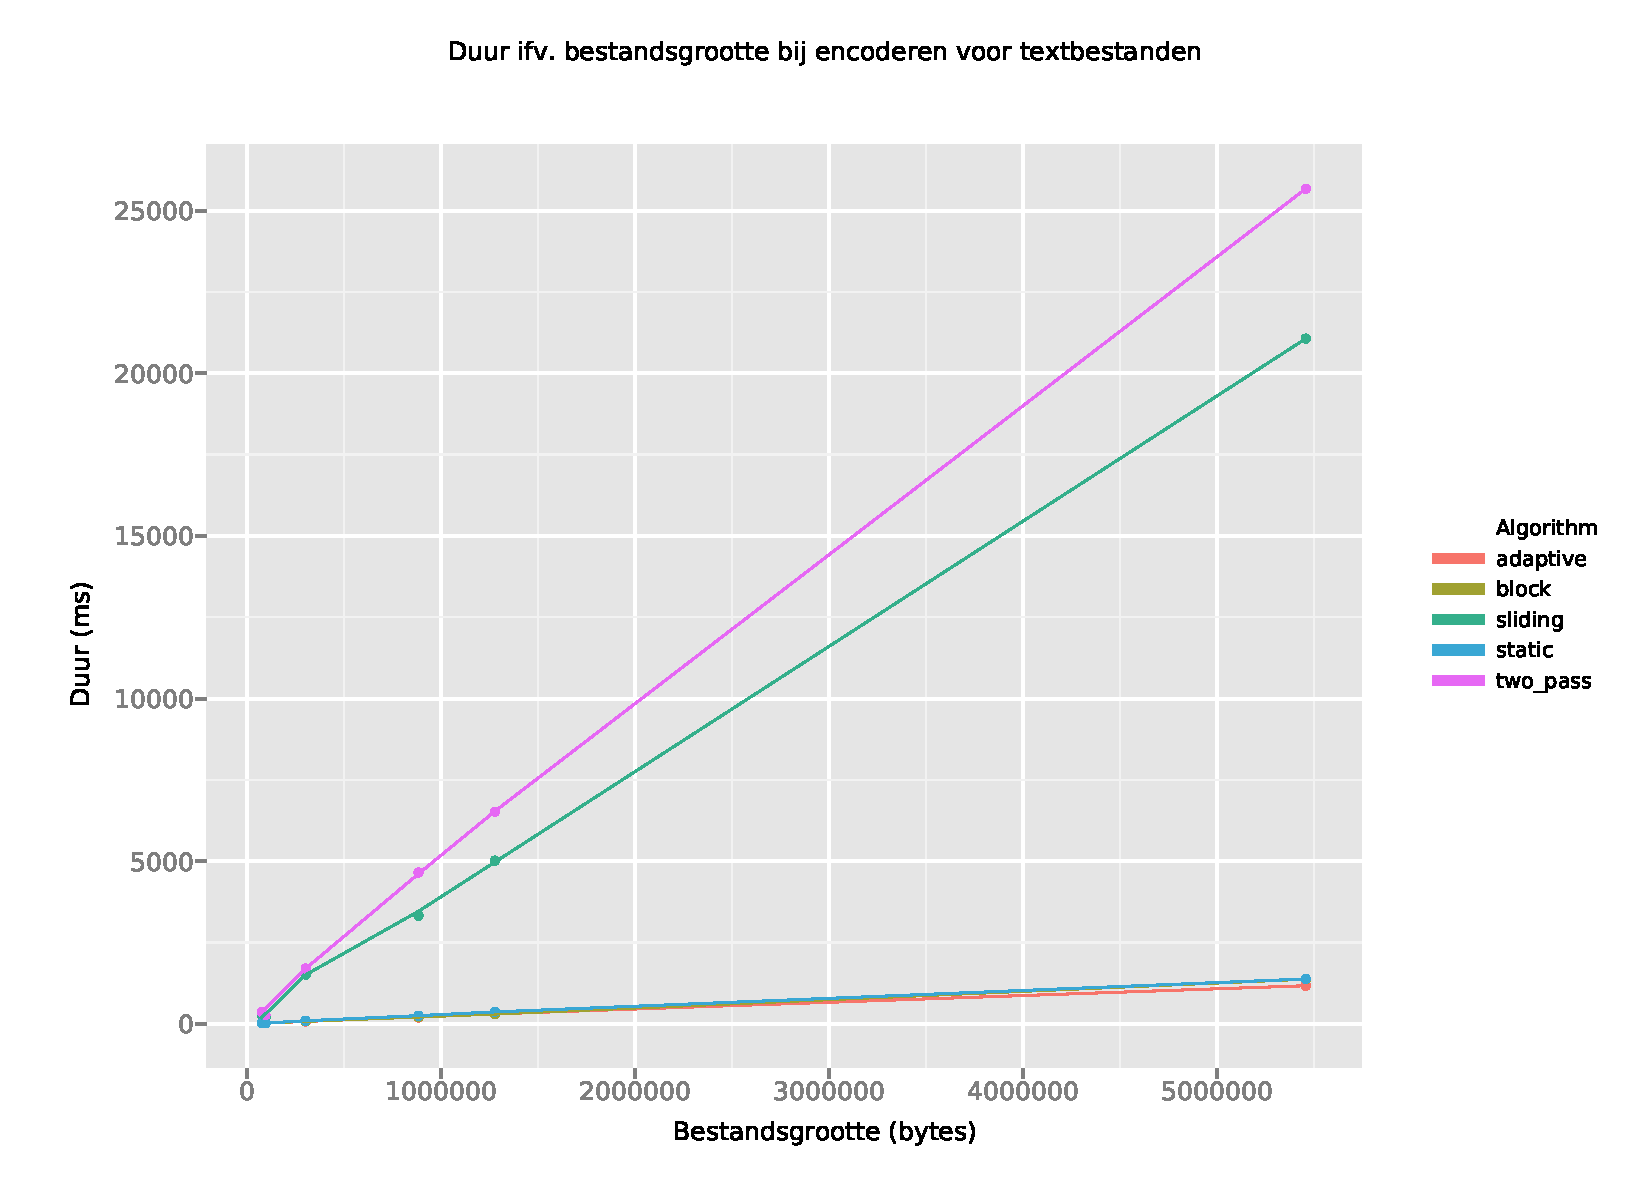
\includegraphics[scale=.6]{../experimenten/grafieken/duur/encode_textbestanden}
\end{figure}
We zien ook dat het 'sliding window' algoritme sneller is dan het 'two pass' algoritme voor tekstbestanden, maar dat het omgekeerde geldt voor binaire bestanden. \\
Dit is te verklaren door het feit dat er bij binaire bestanden veel meer willekeurige bytes zijn. Bij het gebruik van een sliding window kan het dus vaker voorkomen dat er een bepaalde byte meerdere keren uit het window (en dus de boom) verdwijnt. Terwijl we bij het 'two pass' algoritme zeker weten dat elke byte slechts 1 keer verwijderd zal worden.
\begin{figure}[H]
	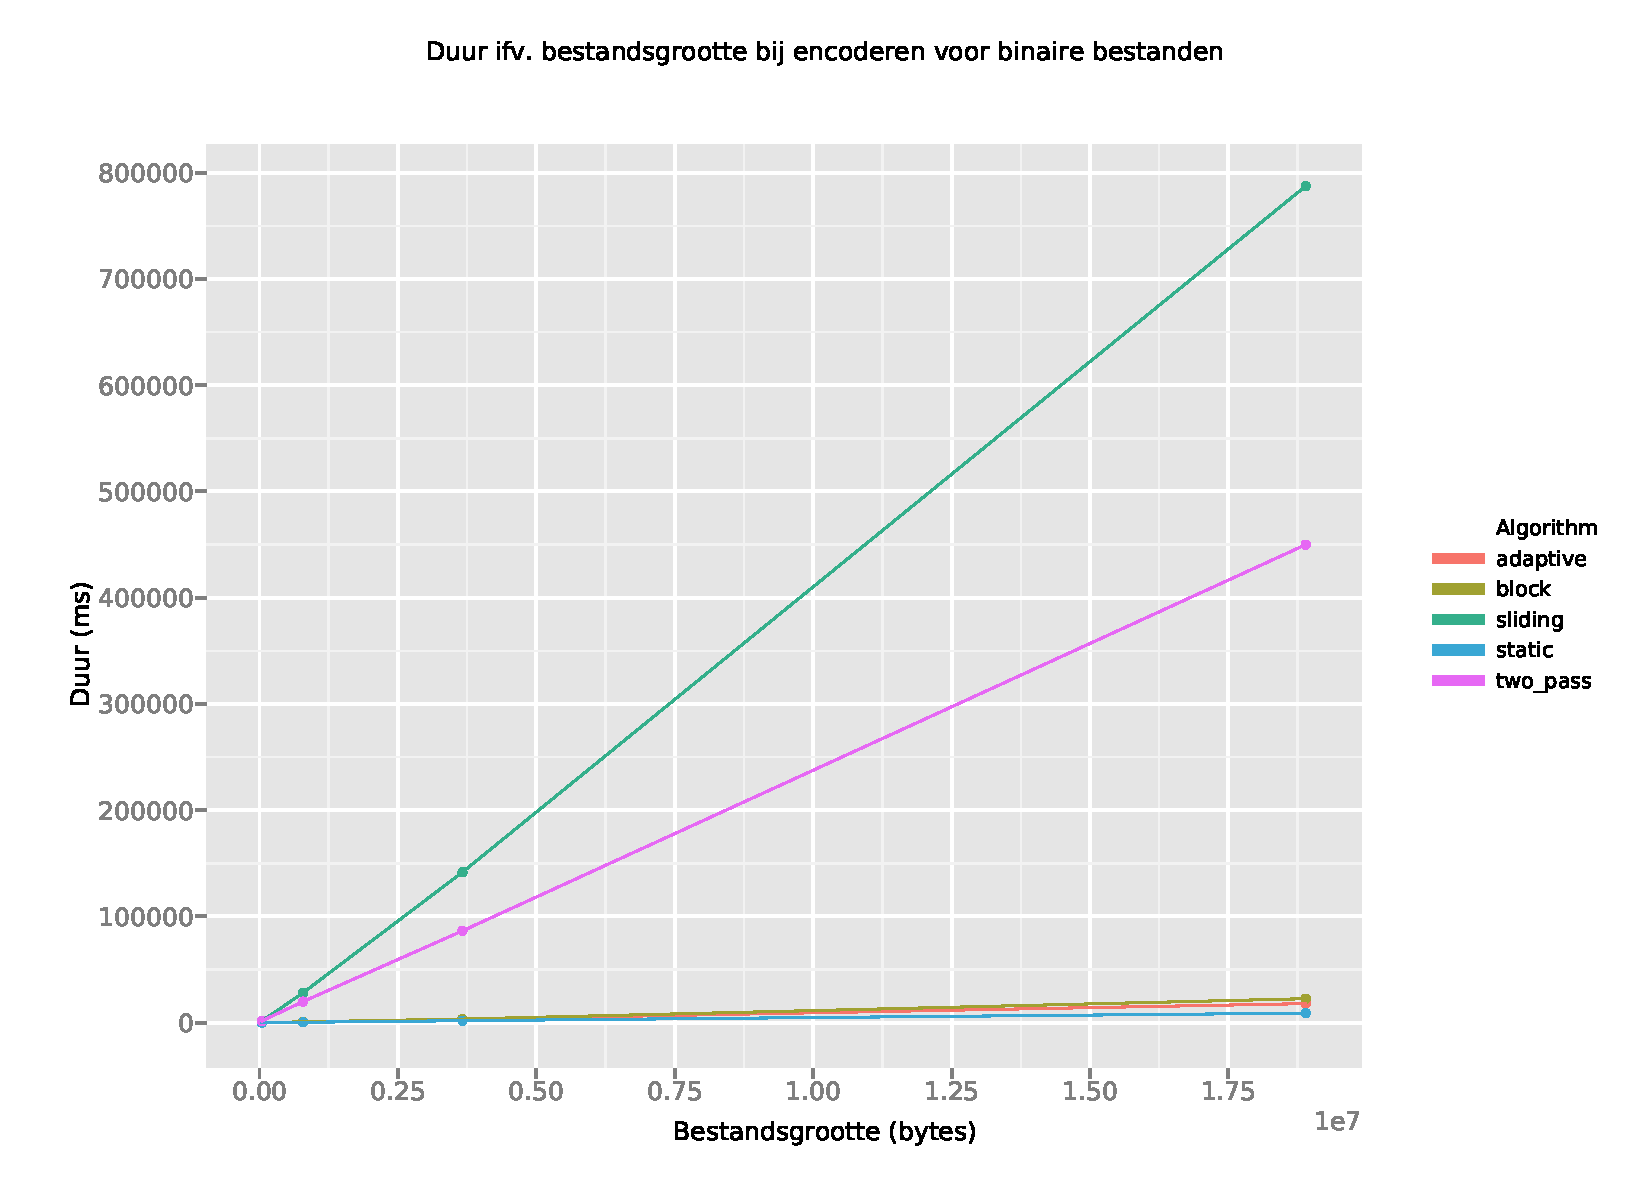
\includegraphics[scale=.6]{../experimenten/grafieken/duur/encode_binaire_bestanden}
\end{figure}
\subsection{Decoderen}
Voor het decoderen zien we gelijkaardige resultaten.
\begin{figure}[H]
	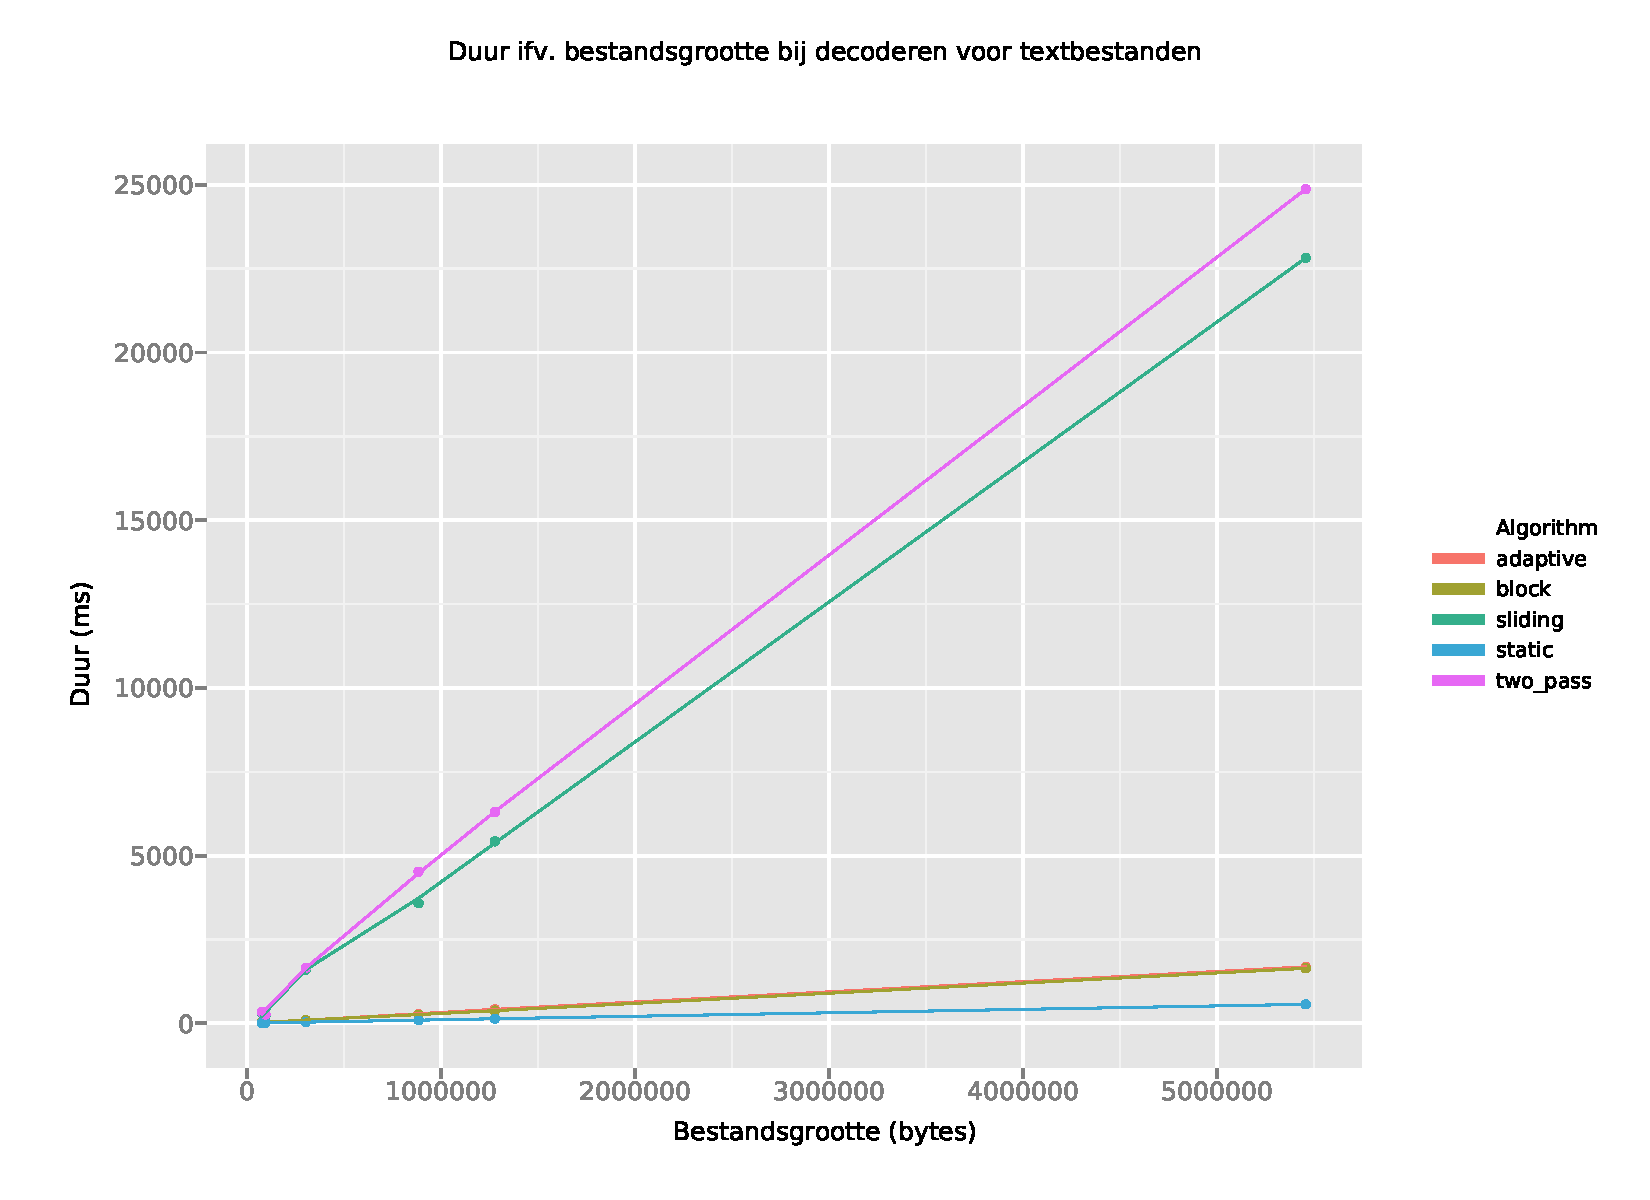
\includegraphics[scale=.6]{../experimenten/grafieken/duur/decode_textbestanden}
\end{figure}
\begin{figure}[H]
	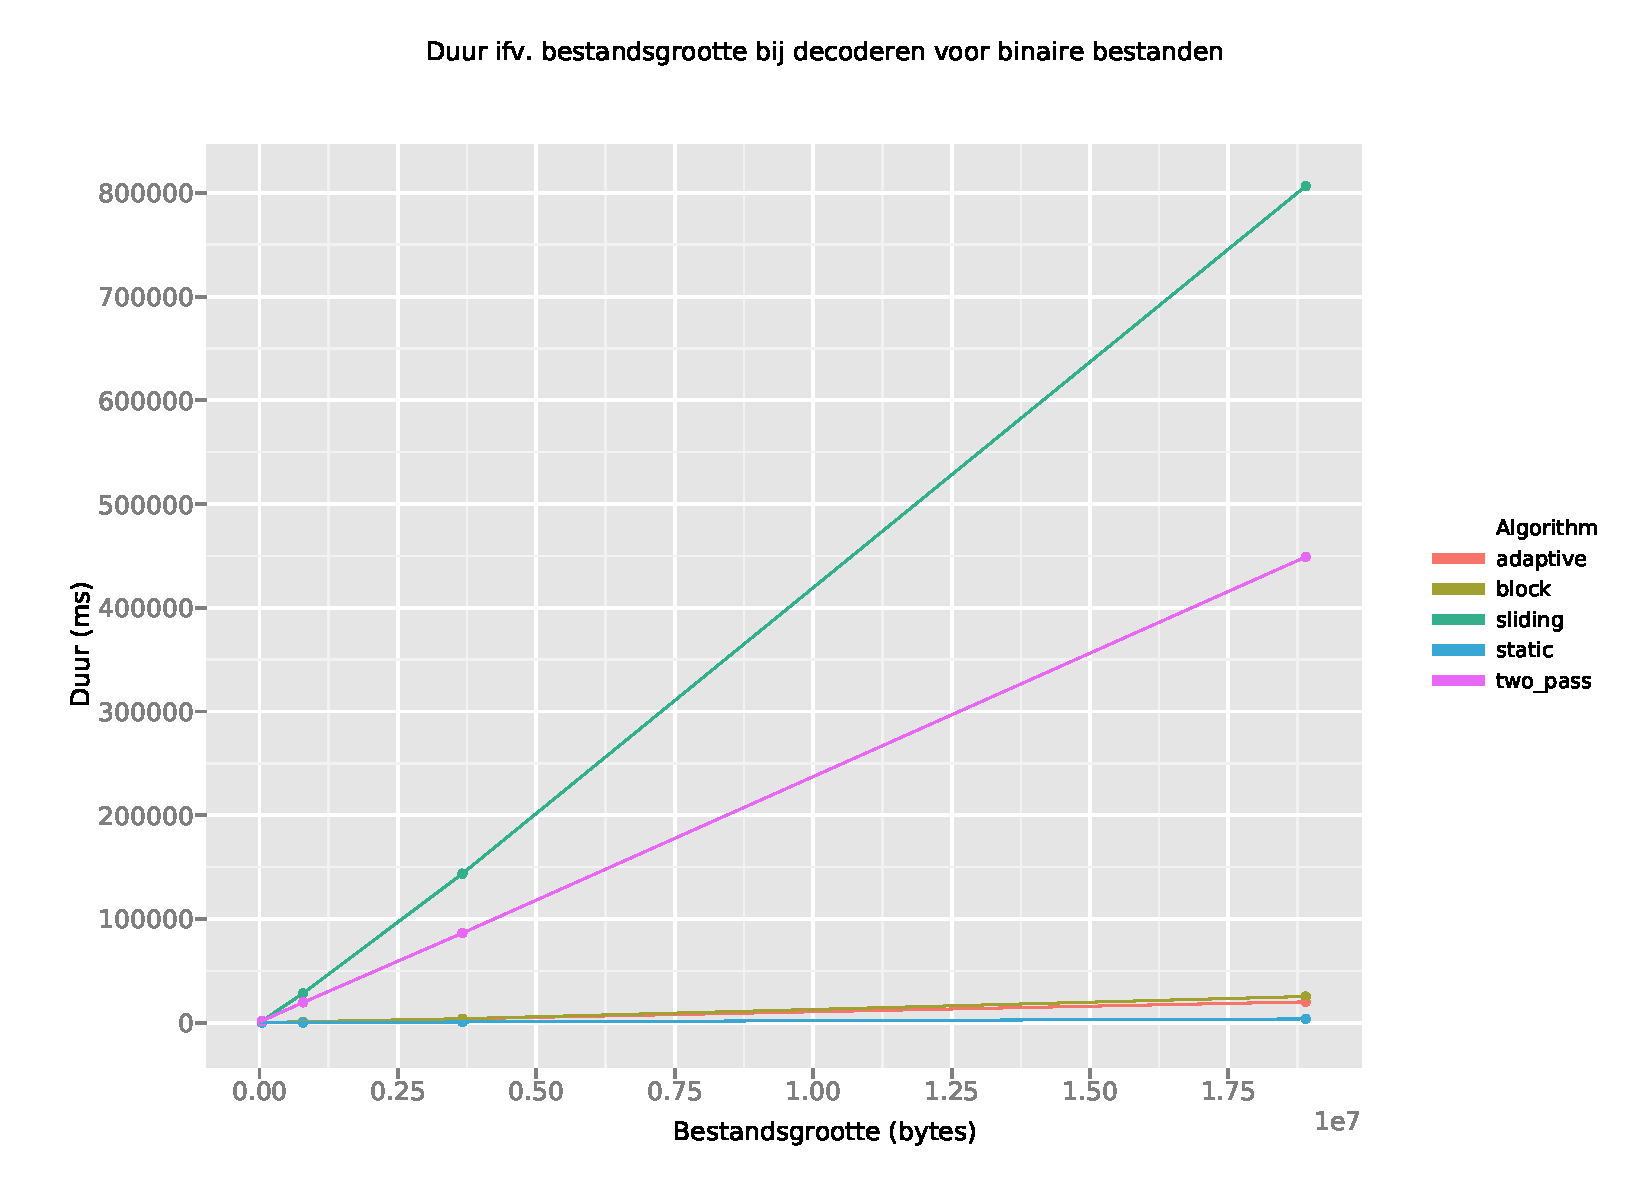
\includegraphics[scale=.6]{../experimenten/grafieken/duur/decode_binaire_bestanden}
\end{figure}
In alle gevallen is het 'statische' algoritme het snelste.
\section{Compressiefactor}
Voor de compressiefactor bekijken we de gemiddelde compressiefactor van de tekstbestanden, de binaire bestanden en het gemiddelde van die twee. \\ \\
Hier zien we effectief dat binaire bestanden veel slechter encoderen dan tekstbestanden. Het 'sliding window' algoritme scoort het beste onder de binaire bestanden, vermoedelijk komt dit omdat het window ervoor zorgt dat de ruimtelijke lokaliteit van de binaire bestanden beter uitgebuit wordt. \\ 
Ook bij tekstbestanden scoort het 'sliding window' algoritme (nipt) het beste.
\begin{figure}[H]
	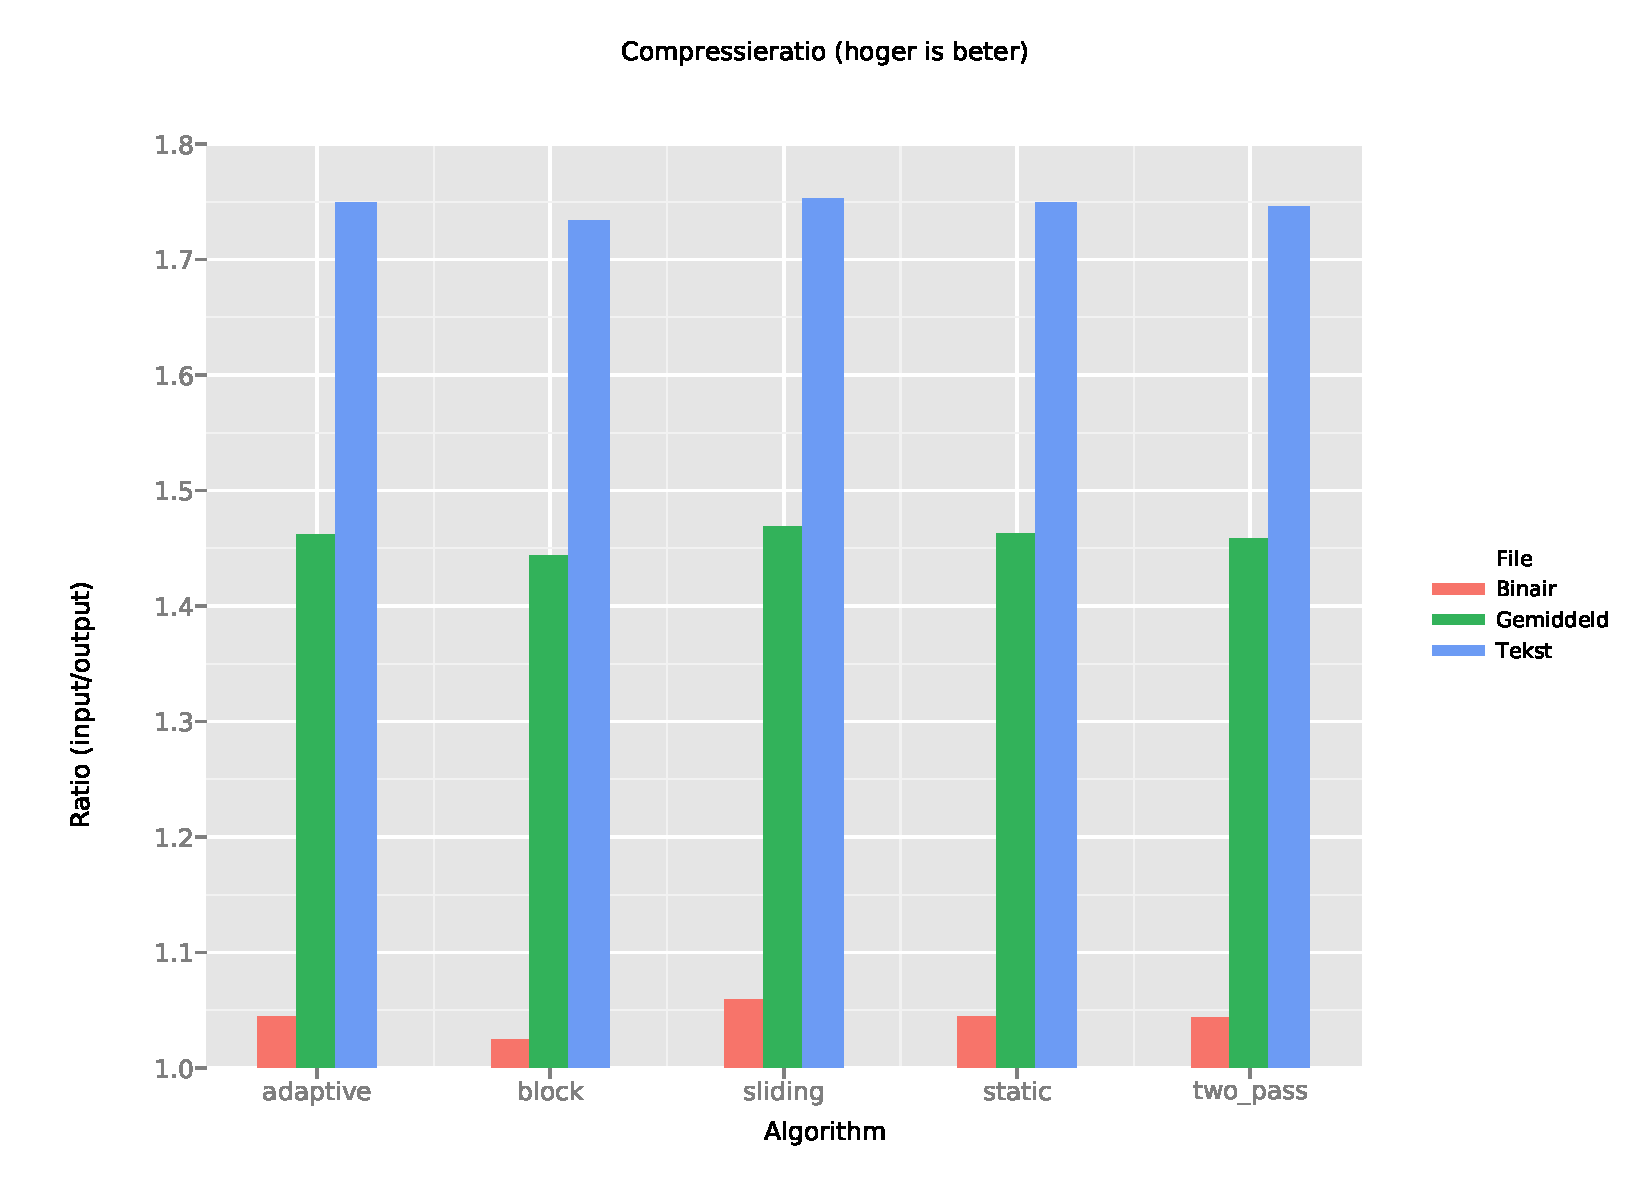
\includegraphics[scale=.6]{../experimenten/grafieken/ratios/ratio}
\end{figure}

\section{Windowgrootte}
Om de ideale windowgrootte te vinden voor de gegeven datasets testen we het encoderen voor een aantal groottes uit.
\begin{figure}[H]
	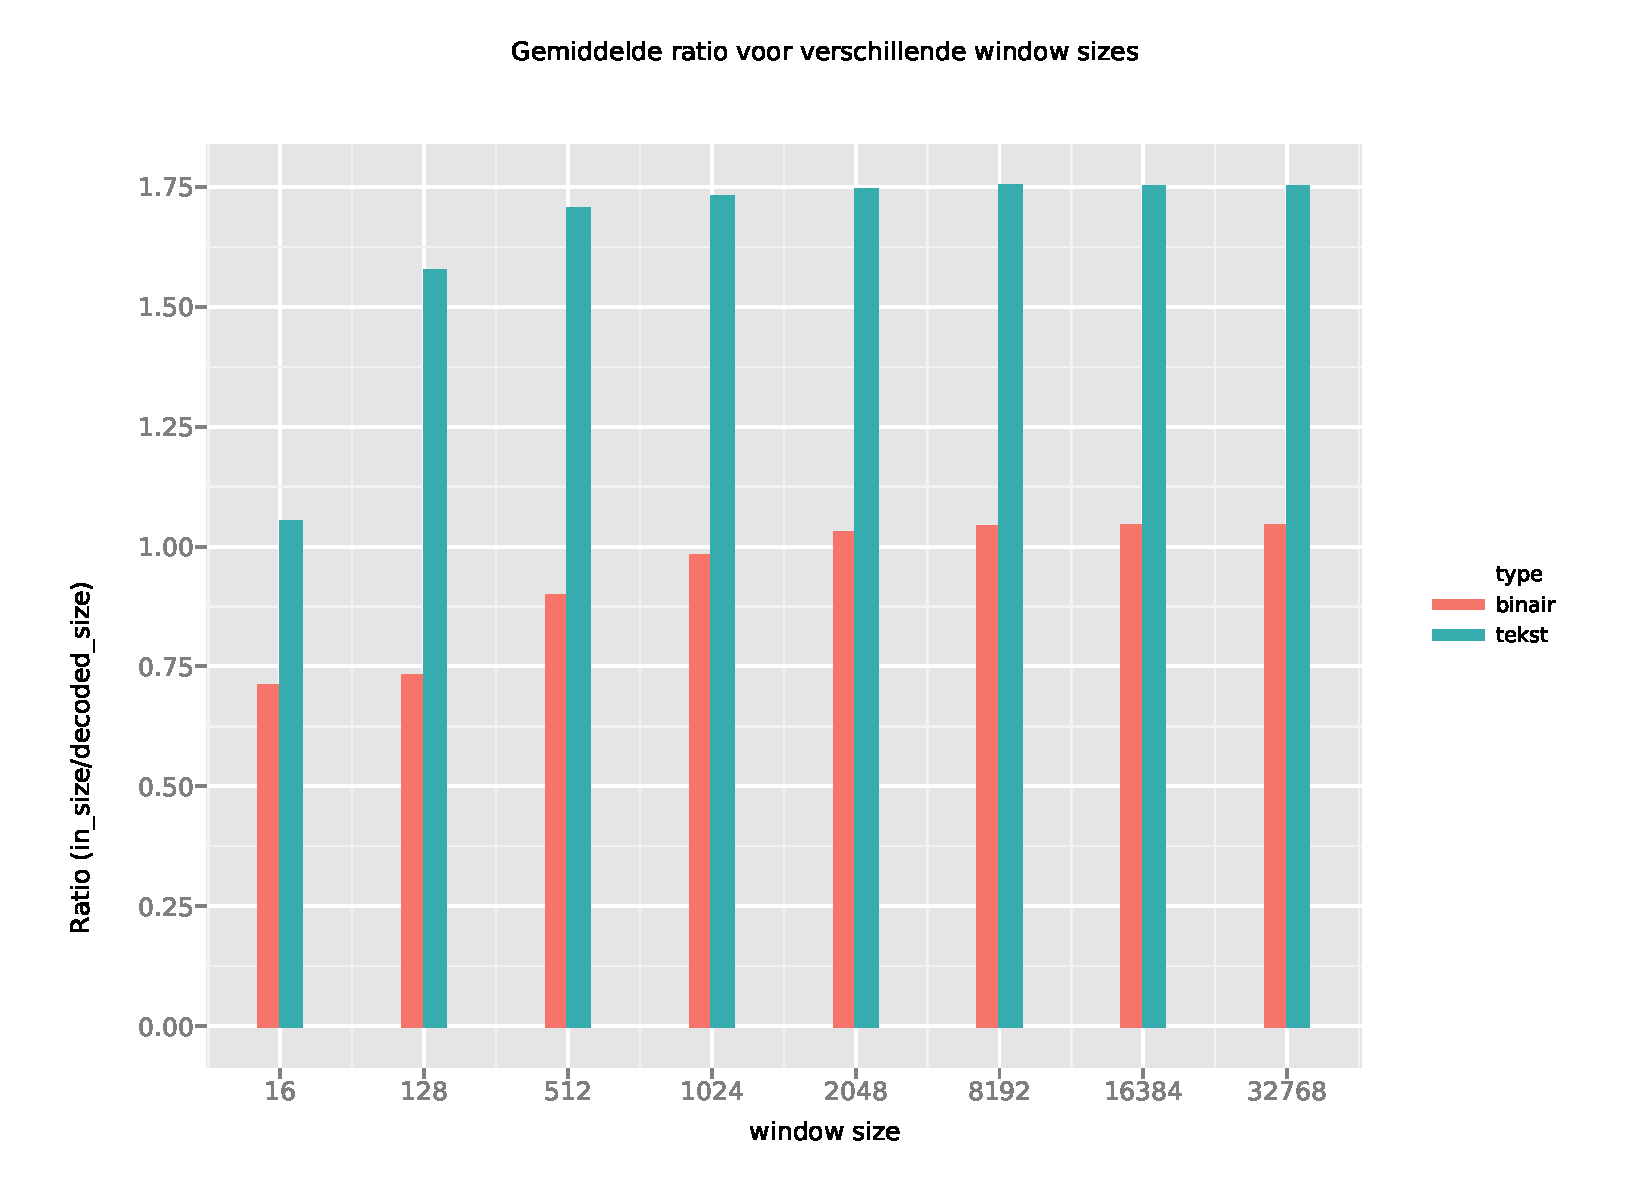
\includegraphics[scale=.6]{../experimenten/window_avg_ratio}
\end{figure}

We zien dat bij een window size van 8192 bytes de optimale compressieratio wordt bereikt voor zowel binaire als tekstbestanden. Kleine window sizes zorgen er zelfs voor dat het bestand groeit bij binaire bestanden omdat de overhead van het algoritme (het uitschrijven van nng) te groot wordt.

\begin{figure}[H]
	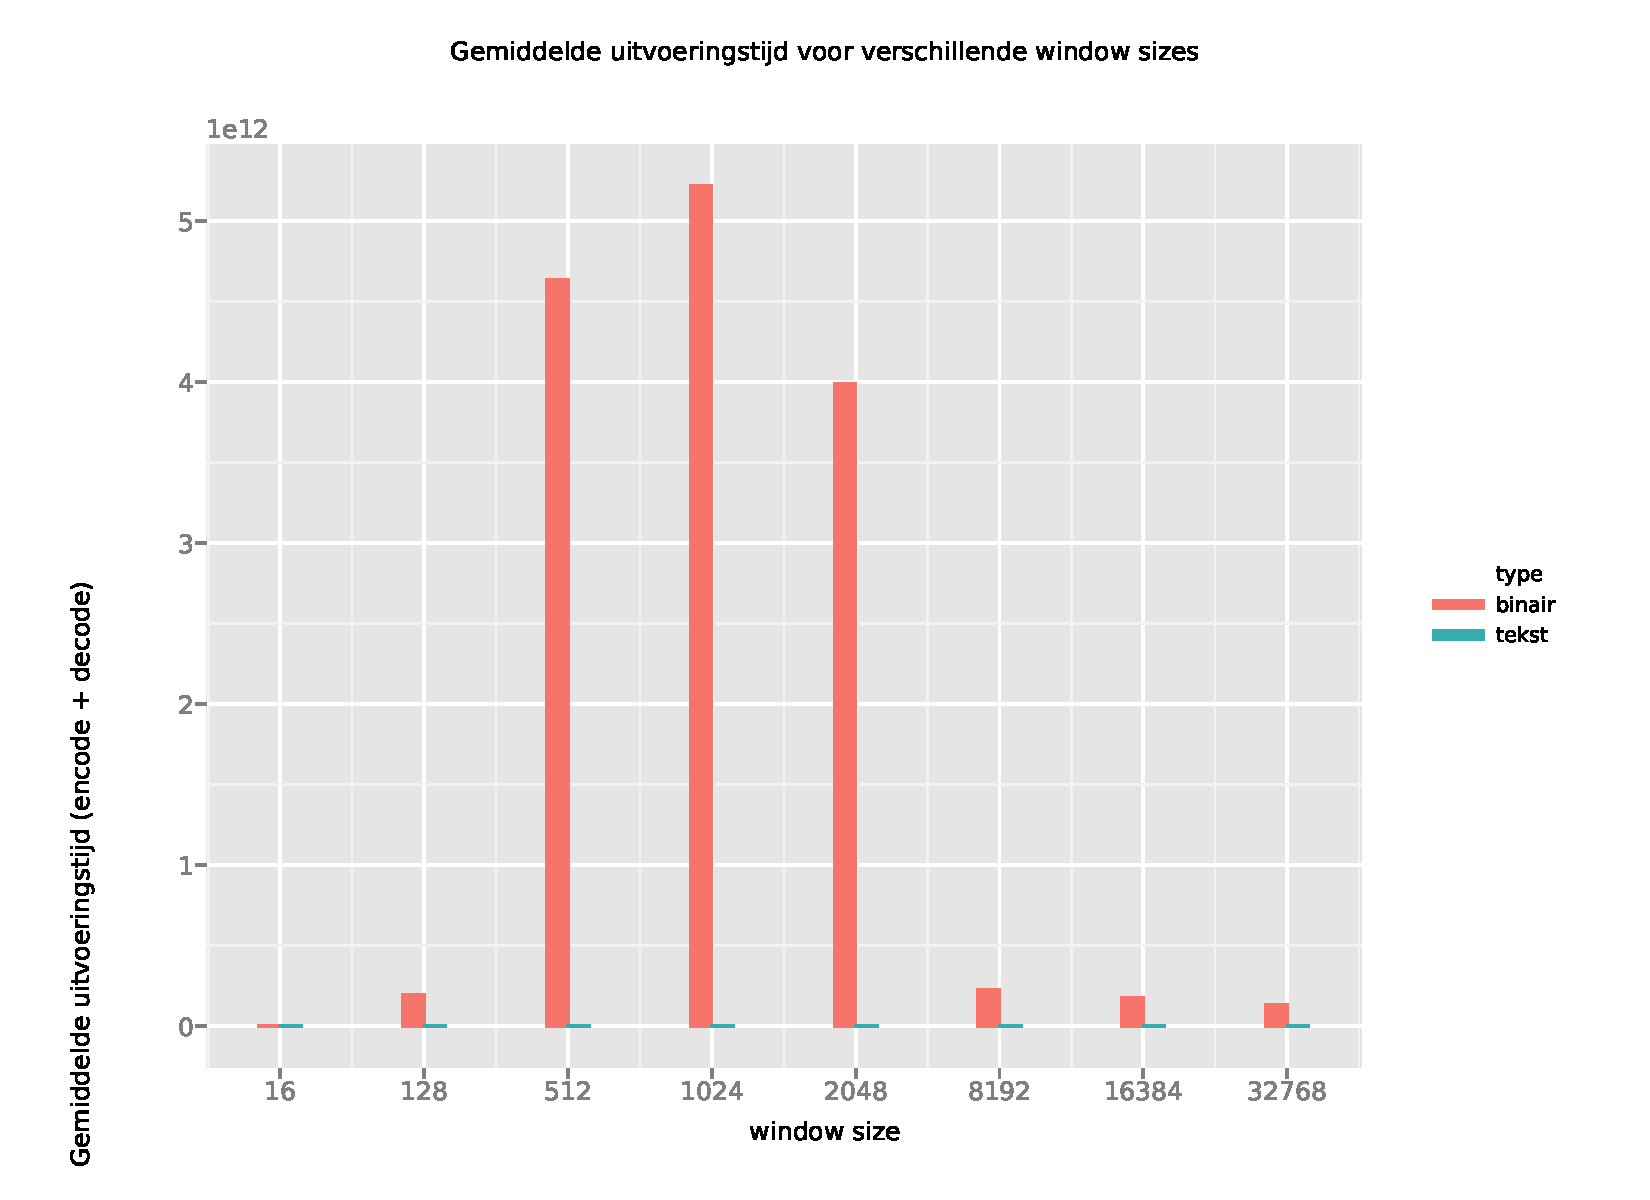
\includegraphics[scale=.6]{../experimenten/window_avg_time}
\end{figure}
Hier merken we op dat bij een window size van 512, 1024 en 2048 bytes het encoderen van binaire bestanden enorm lang duurt. Dit komt vermoedelijk omdat bij het 35MB rockefeller.tiff bestand het window niet genoeg van de dataset in het window kan cachen waardoor er bytes voortdurend uit het window verwijderd worden en nadien opnieuw toegevoegd worden. \\ \\
Bij window sizes van 16bytes en 128bytes vormt dit minder en probleem omdat de boom daar relatief klein blijft en de (dure) \Call{reduceFrequency}{} een stuk goedkoper is. \\ \\
Vanaf 8192bytes zitten de bytes van de 'working set' van het bestand in het window. \Call{delete}{} operaties komen dus minder vaak voor.
\section{Blokgrootte}
Analoog met hierboven kijken we welke blokgrootte voor de gegeven data ideaal is. Dit is niet helemaal hetzelfde als de ideale windowgrootte vinden aangezien er bij elk nieuw blok een volledig nieuwe boom begonnen wordt. We willen dus zoveel mogelijk dezelfde data in een blok krijgen, maar het maakt niet uit waar de data binnen het blok zich bevindt. \\
\begin{figure}[H]
	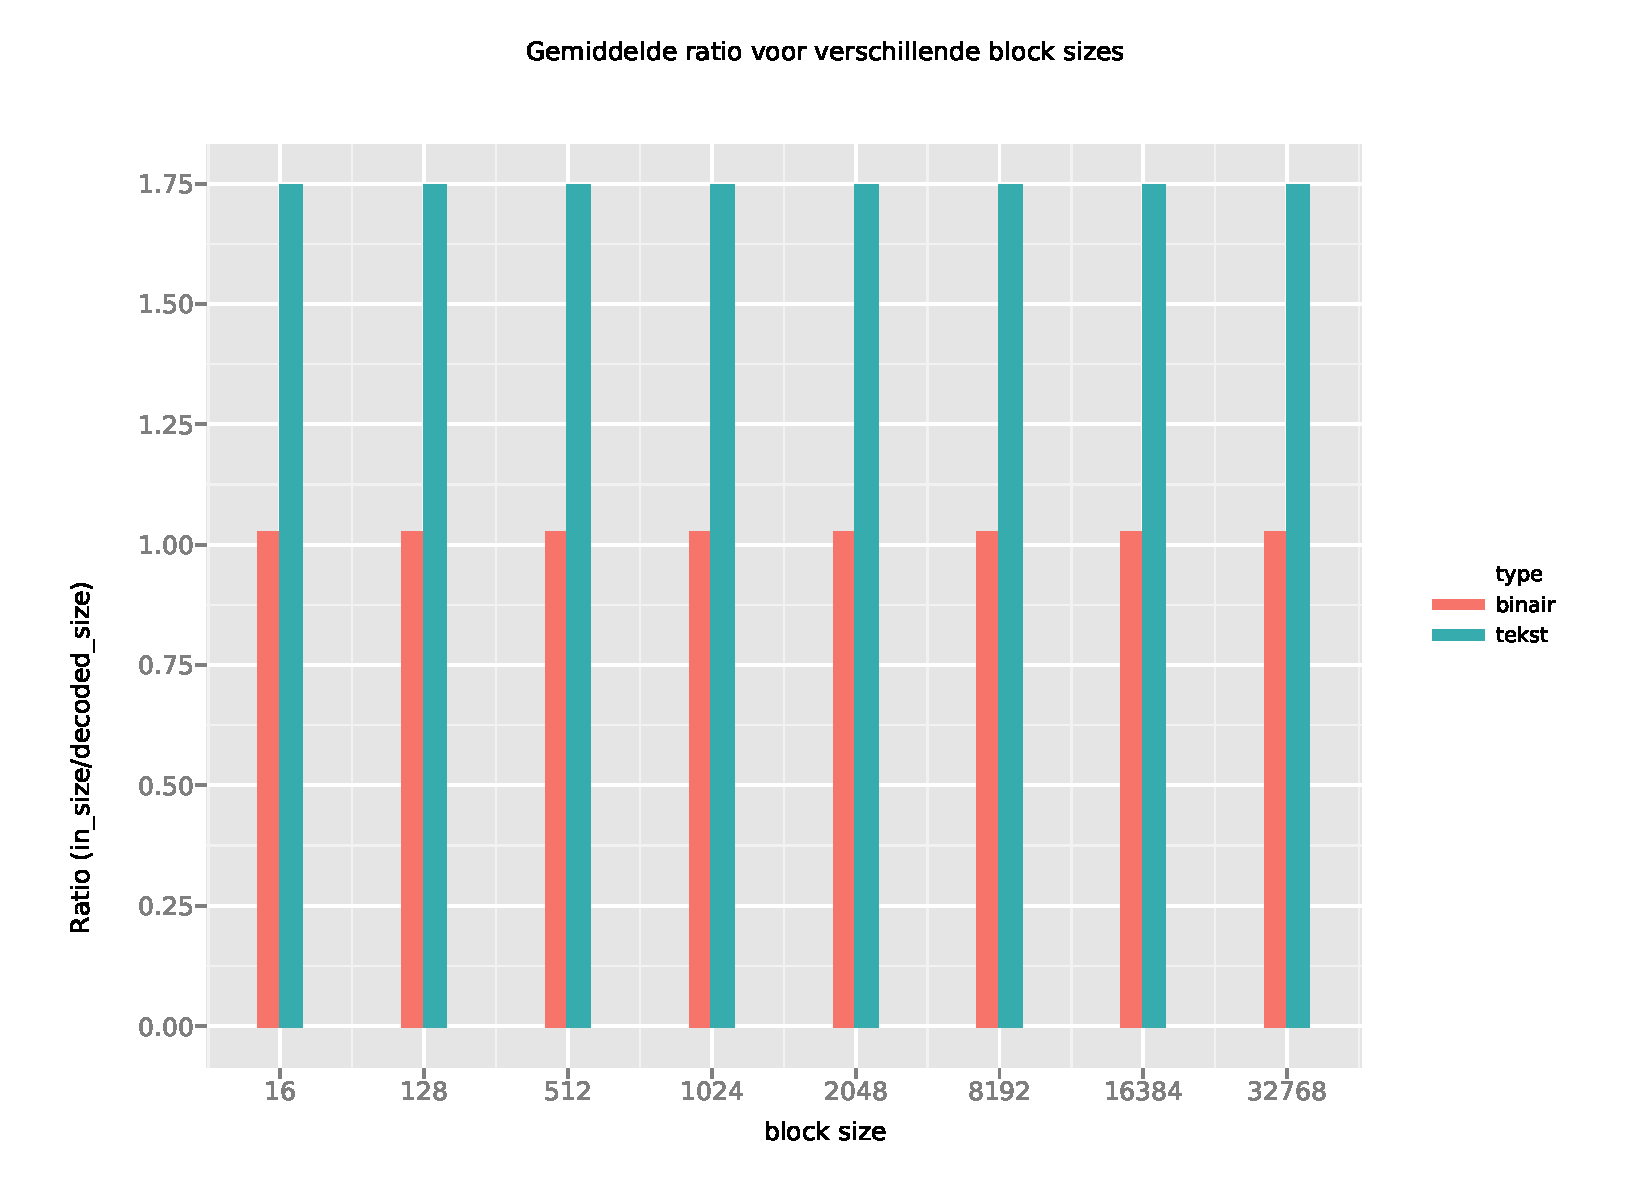
\includegraphics[scale=0.6]{../experimenten/block_avg_ratio}
\end{figure}
We zien dat onafhankelijk van de blokgrootte de compressiefactor ongeveer hetzelfde blijft.  
\begin{figure}[H]
	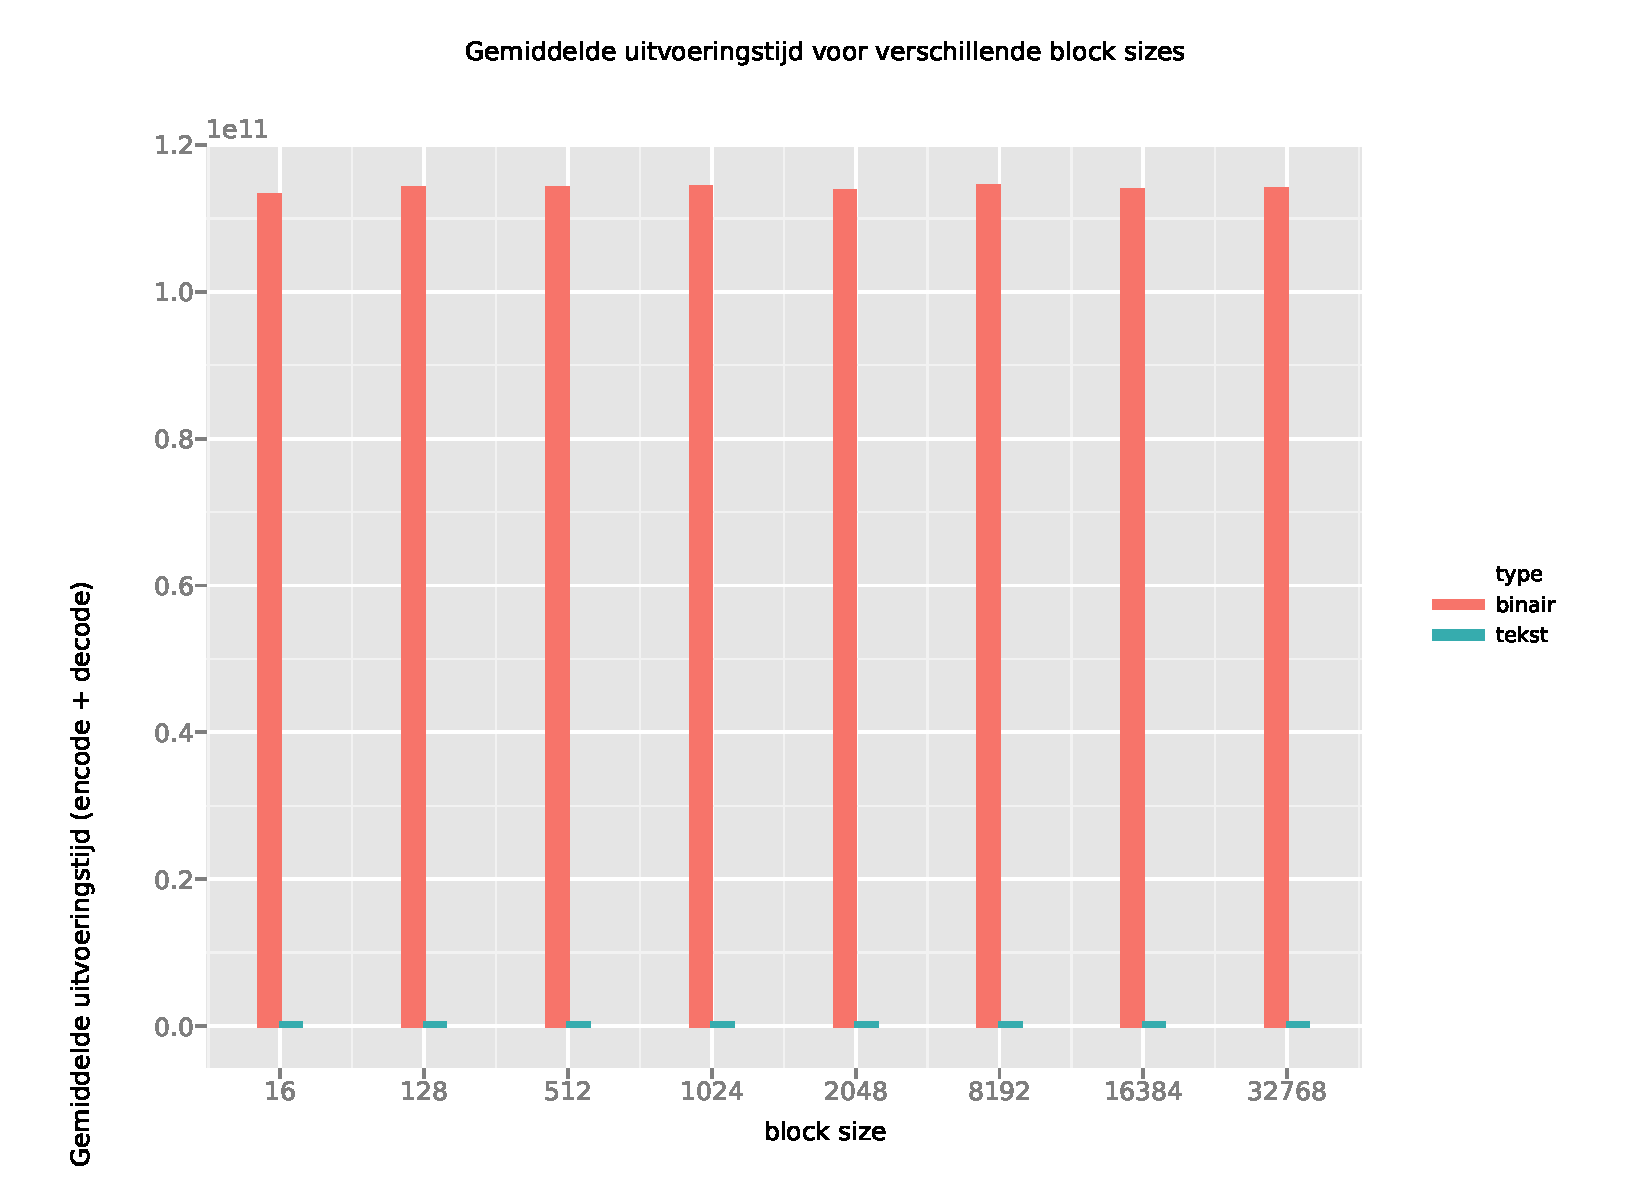
\includegraphics[scale=0.6]{../experimenten/block_avg_time}
\end{figure} 
Ook het encoderen van binaire bestanden duurt langer dan het encoderen van tekstbestanden, maar ook hier merken we op dat onafhankelijk van de blokgrootte het encoderen ongeveer even lang duurt.
\section{Optimale datasets}
\subsection{Sliding}
We merken op dat het sliding algoritme voor dit soort datasets ongeveer 4x beter werkt dan de andere algoritmen. Ook zien we, zoals we eerder vermoedden, dat het bloksgewijze algoritme ook ongeveer even goede prestaties heeft.
\begin{figure}[H]
	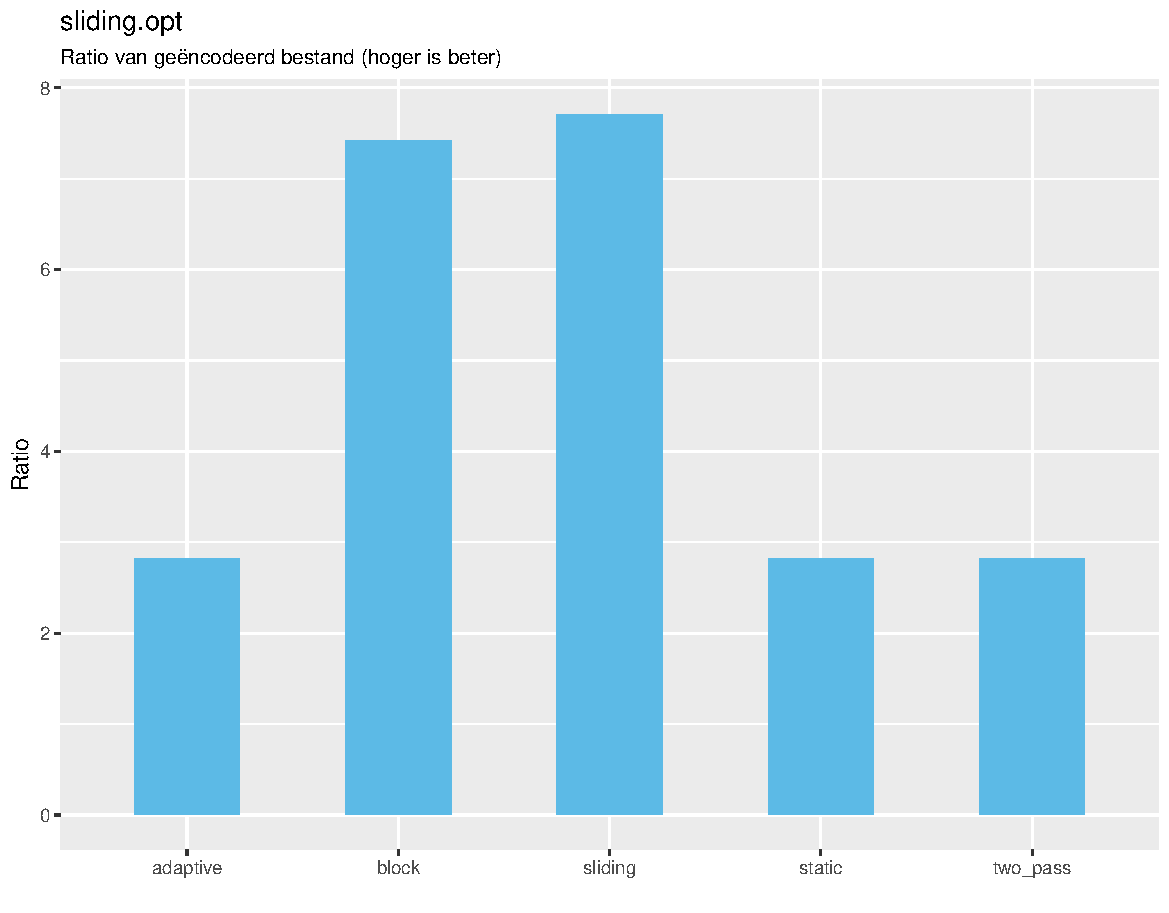
\includegraphics[scale=0.8]{../experimenten/grafieken/sliding_opt}
\end{figure}

\subsection{Two pass}
Bij deze dataset merken we op dat het verschil tussen de verschillende algoritmen erg klein is. Het sliding algoritme heeft hier de beste prestaties. Het two pass algoritme scoort wel net iets beter dan de andere algoritmen. Als we het bestand dus enkele ordes groter zullen maken zou dit wel een verschil kunnen maken.
\begin{figure}[H]
	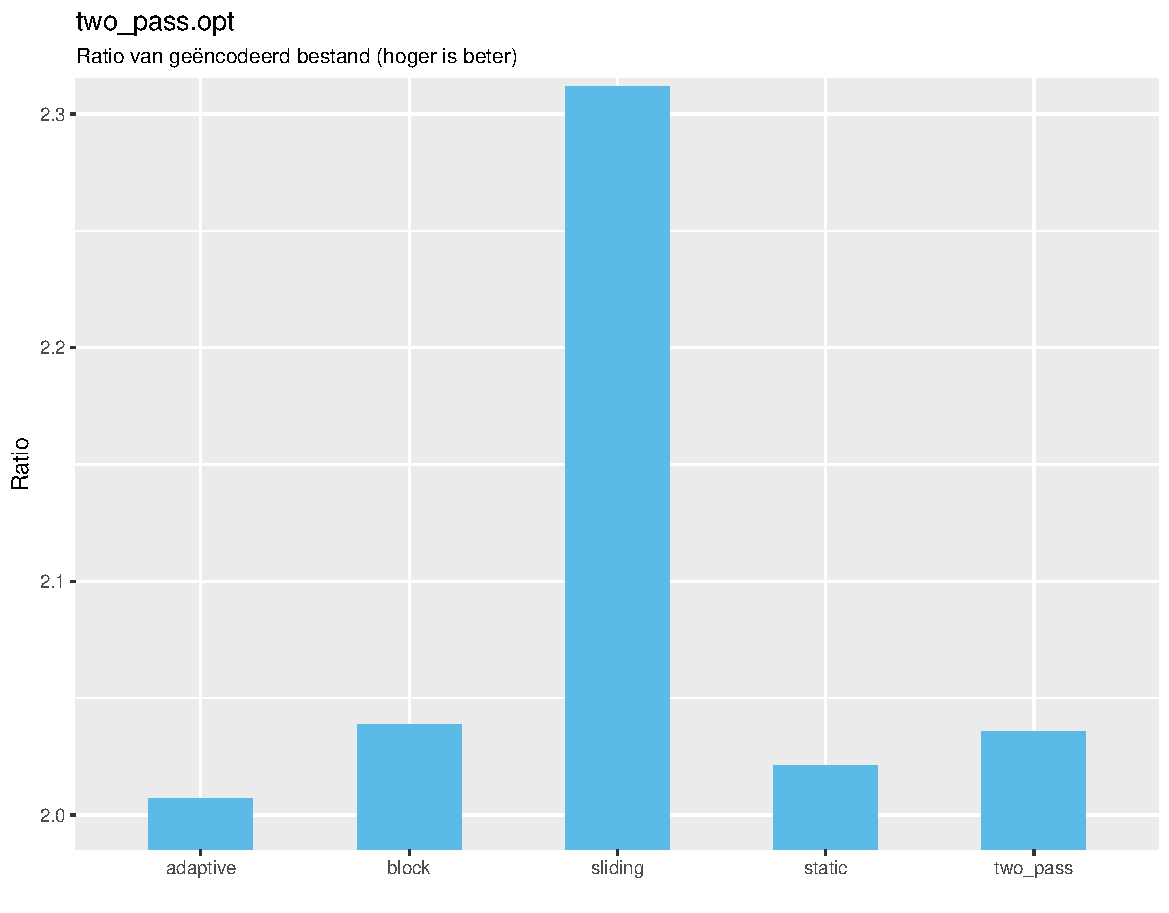
\includegraphics[scale=0.8]{../experimenten/grafieken/two_pass_opt}
\end{figure}

\chapter{Besluit}
%%%%%Statisch
\section{Statische huffman}
Het statische algoritme is in elk geval het snelste algoritme van alle geteste algoritmen. Dit is het grootste voordeel. \\ \\
Een ander voordeel is dat statische huffman redelijk bestand is tegen transmissiefouten, indien er ergens een bitfout optreedt heeft dit minder dramatische gevolgen dan bij de andere algoritmen aangezien de boom niet dynamisch opgebouwd wordt. \\ \\
Een nadeel van het statische huffman algoritme is echter het feit dat de tekst 2x doorlopen moet worden en online encoderen dus niet mogelijk is. \\ \\
Een ander nadeel is dat de boom afzonderlijk moet opgeslagen worden en dit voor extra overhead kan zorgen in het bestand. In de praktijk hebben we echter waargenomen dat deze overhead ongeveer even groot is in vergelijking met de andere algoritmen (door de beperking op de alfabetgrootte en de overhead die andere algoritmen hebben).
%%%%%Adaptive huffman
\section{Adaptive huffman}
Het grootste voordeel van dit algoritme (alsook de volgende algoritmen) is dat de boom dynamisch wordt opgebouwd, dit algoritme is dus online. \\ \\
Nog een voordeel is dat de boom niet afzonderlijk opgeslagen hoeft te worden en opgebouwd wordt naargelang de bytes komen (idem voor onderstaande algoritmen). \\ \\
Een nadeel van dit algortime is dat de huffman-boom optimaal is voor de voorbije bytes en niet de komende bytes. In het geval dat een eerder frequent voorkomende byte dus niet meer voorkomt, zal deze nog steeds relatief hoog in de boom blijven staan. Voor tekstbestanden komt dit geval echter niet vaak voor. \\ \\
Ook is dit algoritme (en de volgende algoritmen) erg gevoelig voor bitfouten. 1 fout kan ervoor zorgen dat de rest van de tekst volledig ondecodeerbaar wordt.

%%%%%%%%Adaptive huffman met sliding window
\section{Adaptive huffman met sliding window}
Deze boom is nog altijd optimaal voor de voorbije bytes, maar het 'frame of reference' van het sliding window algoritme een stuk kleiner, waardoor de informatie in het window vaak nog relevant is voor de komende bytes. \\ \\
Voor binaire bestanden kunnen we de huffman-boom als een soort cache beschouwen. Net als bij caches zal een kleinere boom de byte effici\"enter kunnen coderen maar een cache misser zal altijd duur zijn. Indien we een goede balans van de cachegrootte kunnen vinden waar de window size groot genoeg is om ruimtelijke lokaliteit uit te buiten, maar het window niet zo groot is dat de huffman-boom te groot wordt, dan zullen we een optimale window size bereiken. \\ \\
Een ander voordeel van het sliding window algoritme is dat er bytes uit de boom kunnen verdwijnen, de codes zullen dus over het algemeen korter zijn dan wanneer dit niet kan. \\ \\
Het grootste nadeel van dit algoritme is dat dit algoritme relatief traag is door de \Call{reduceFrequency}{} operatie. Indien een suboptimale window size wordt gekozen kan dit het algoritme zelfs vele malen trager maken omdat er continu bytes verwijderd en opnieuw toegevoegd worden.
%%%%%Two pass
\section{Two pass adaptive huffman}
Het grootste voordeel van two pass adaptive huffman is dat de boom optimaal is voor de bytes die nog moeten volgen.\\ 
In de praktijk zal dit echter niet veel verschil maken omdat bij tekstbestanden de voorbije bytes een goede referentie vormen voor de bytes die nog moeten komen. Bij binaire bestanden buit het 'sliding window' algoritme dan weer de lokaliteit beter uit, waardoor 'two pass' ook hier slechter(/even goed) scoort dan de andere algoritmen. \\ \\
Een nadeel is dat dit algoritme ook weer relatief traag is, dit omdat we weten dat elke character uit de boom zal verwijderd moeten worden. \\ \\
Hier moet de tekst 2x doorlopen worden bij het encoderen. Maar bij het decoderen is dit niet noodzakelijk (we moeten niet verder kijken om te zien hoeveel bits we op het einde moeten negeren).
%%%%%Bloksgewijze adaptive huffman
\section{Bloksgewijze adaptive huffman}
Het bloksgewijze algoritme presteert qua compressie net iets minder goed dan de andere algoritmen. Maar daartegen staat dat het algoritme erg schaalbaar is, in principe zouden er een erg groot aantal symbolen (van meer dan 1byte bijvoorbeeld) en een oneindig grote dataset kunnen gebruikt worden en zou dit algoritme nooit problemen met het geheugen krijgen, een luxe die er bij statische huffman bvb. niet is. \\ \\
In theorie kan dit algoritme ook sneller werken dan adaptive huffman indien er heel veel verschillende bytes voorkomen en de blokgrootte zo gekozen wordt dat grote huffman-bomen vermeden worden. \\ \\
Dit algoritme werkt ook ongeveer met hetzelfde principe als het 'sliding window' algoritme (met een ander doel), echter is het veel sneller omdat na elke blok de boom volledig opnieuw opgebouwd wordt en de characters niet telkens verwijderd moeten worden. Natuurlijk is er hierdoor wel wat meer overhead. \\ \\ 
Wanneer we headers zouden gebruiken tussen de verschillende blokken zouden we er zelfs voor kunnen zorgen dat een bitfout slechts 1 blok corrupt maakt. Wat 'bloksgewijze adaptieve huffman met headers' dus een practischer algoritme zou maken dan het gewone 'adaptive huffman' algoritme als de data over een kanaal met veel ruis verstuurd zou moeten worden. \\ 
Ook kunnen we wanneer we headers gebruiken de tekst parallel encoderen en decoderen indien we nog enkele wijzigingen aan het algoritme zouden maken.\\ \\
Wanneer we de blokgrootte groter maken zal de overhead per blok lager liggen omdat er in totaal minder vaak een 'nng' zal voorkomen, natuurlijk verliezen we vanaf een bepaalde blokgrootte de hiervoor genoemde voordelen.

\chapter{Wijzigingen aan de code sinds het indienen op 1/12}
\begin{itemize}
	\item Er ontbrak nog een cast naar \textbf{unsigned char} bij het statische huffman algoritme. Dit had als gevolg dat bij het encoderen van binaire bestanden er segfaults konden optreden. Bij ASCII bestanden kwamen deze fouten niet voor omdat de char waarde tussen 0 en 127 ligt en dus niet negatief gaat.
	\item Om verschillende blok/window-grootten te kunnen testen werd de '-s' parameter toegevoegd waarmee een custom blok/window size kan meegegeven kan worden die dan de standaardgrootte zal overschrijven (1024).
\end{itemize}
%%%%%Bloksgewijze adaptive huffman
\end{document}